%!TEX TS-program = pdflatex
%!TEX root = progetto_finale.tex
%!TEX encoding = UTF-8 Unicode

\chapter{Progetto} \label{progetto}

In questo capitolo vengono descritte l'architettura del software, i protocolli e gli algoritmi utilizzati, l'architettura fisica e il piano di sviluppo.

This chapter is devoted to the description of the general architectures, and specific algorithms.

\section{Architettura Logica}
Describe the components of your systems: modules/objects/components/services. For each component, describe the functionalities it implements, and by who is used.

\begin{itemize}
	\item Modulo algoritmi grafi: fornisce gli algoritmi che è possibile utilizzare sui grafi. Per esempio include Dijkstra, BFS, DFS, aggiungi nodo, aggiungi arco, ... 
	
	\item Modulo per l'algoritmo di elezione del leader: implementa la funzionalità della scelta della macchina da assegnare all'utente.
	
	\item Modulo per l'invio di messaggi: controlla che il messaggio sia ben formato.
	
	\item Modulo interfaccia cliente-servizio: fornisce le possibili operazioni che un cliente può richiedere al sistema.
	
	\item Modulo scheda wireless: simula la scheda di rete che fornisce i vicini dell'entità che ne invoca i metodi.
	
	\item Modulo mappa città: fornisce i metodi di lettura e modifica della mappa della città.
	
	\item Modulo gestione macchine: fornisce i metodi per ricaricare le batterie delle macchine, ne gestiscono gli incidenti e le riparazioni.
	
	\item Modulo creazione entità: fornisce le primitive per creare nuove macchine e nuovi utenti.
	
	\item Modulo comunicazione Ambiente-Entità: il processo Ambiente può utilizzare i metodi in questo modulo per simulare il mondo reale.
	
	\item Modulo Entità Macchina: rappresenta l'astrazione dell'entità veicolo.
	
	\item Modulo Entità Utente: rappresenta l'astrazione dell'entità utente.

\end{itemize}

Per rappresentare il comportamento delle entità coinvolte in base ai possibili eventi, sono stati creati due automi che rappresentano i possibili stati delle macchine e degli utenti. In essi, gli stati sono rappresentati da degli ovali, mentre gli eventi da dei riquadri di colore blu o rosso. Queste tonalità esprimono il tipo di messaggio: ricezione ed invio.

L'immagine \ref{fig:automa_utente} rappresenta l'automa degli stati dell'entità utente e come esso cambia il proprio stato in base agli eventi e messaggi.


\begin{figure}[htbp]
	\centering
	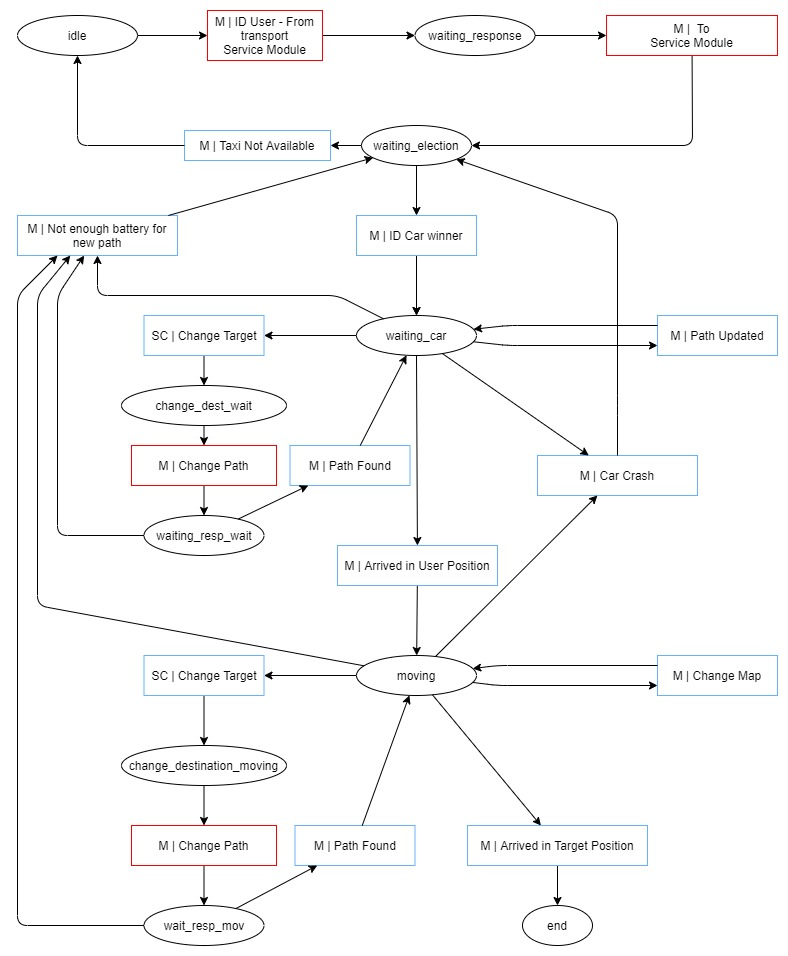
\includegraphics[width=15cm]{automa_utente.jpg}
	\caption{Rappresentazione degli stati possibili dell'entità utente.}
	\label{fig:automa_utente}
\end{figure}

L'immagine \ref{fig:automa_macchina} rappresenta l'automa degli stati dell'entità macchina e come esso cambia il proprio stato in base agli eventi e messaggi.


\begin{figure}[htbp]
	\centering
	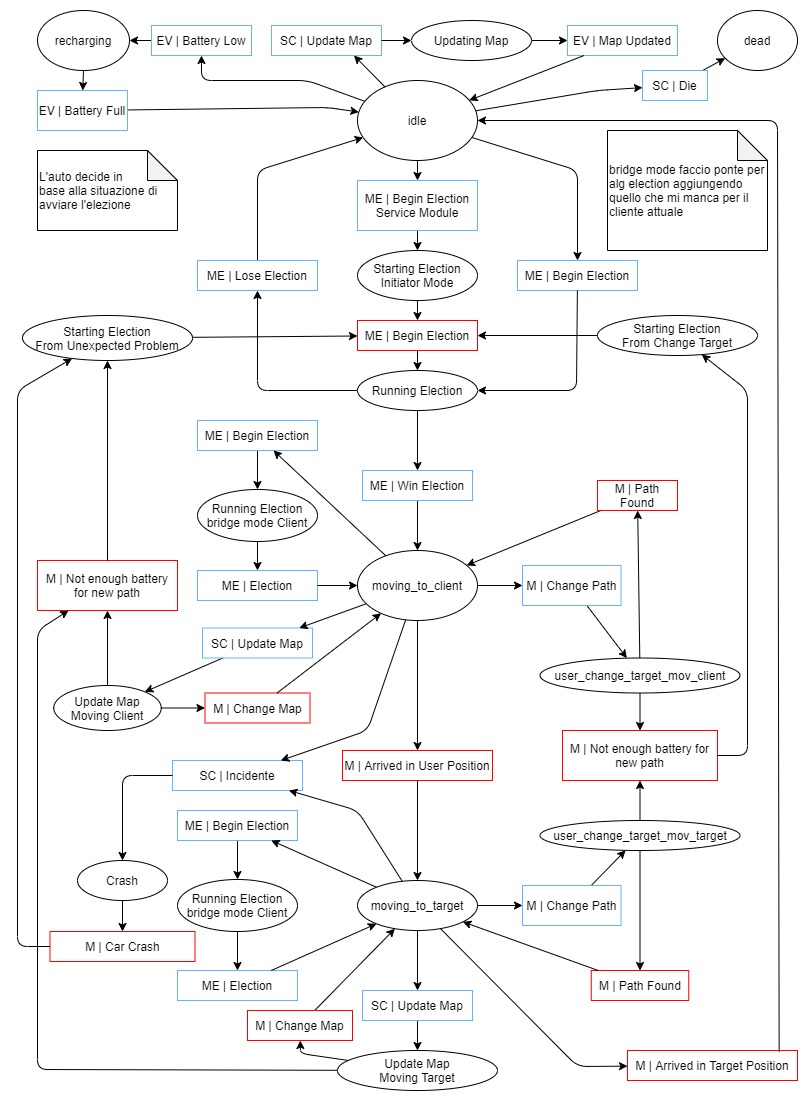
\includegraphics[width=15cm]{automa_macchina.jpg}
	\caption{Rappresentazione degli stati possibili dell'entità macchina.}
	\label{fig:automa_macchina}
\end{figure}

\newpage

\section{Protocolli e algoritmi}
In questa sezione vengono discusse le comunicazioni tra le diverse componenti e gli algoritmi utilizzati all'interno del sistema.

\subsection{Funzioni di costo delle macchine} \label{funzioni_di_costo_macchine}
Per la scelta della macchina più adatta, vengono considerati i seguenti parametri.

\begin{itemize}
	\item Crdt = Carica Rimanente Dopo Trasporto dell'utente.
	\item Cc = Costo Cliente, esprime dopo quanto tempo la macchina raggiungerebbe il cliente.
	\item Cr = Carica Rimanente espressa in unità di misura della distanza percorribile.
	\item Prc = Percorso Rimanente Cliente espresso in unità di misura della distanza assumendo che il taxi sia occupato.
	\item Pvcn = Percorso Verso Cliente Nuovo a partire dalla posizione dopo lo scorso cliente espresso in unità di misura della distanza.
	\item Pvdc = Percorso Verso Destinazione Cliente a partire dalla posizione attuale del cliente espresso in unità di misura della distanza.
	\item Pvcr = Percorso Verso Colonnina Ricarica per permettere alla macchina di ricaricarsi dopo il trasporto se necessario.
\end{itemize}

\begin{equation} \label{funzione_costo_raggiungimento_cliente}
Cc = Prc + Pvcn
\end{equation}

\begin{equation} \label{carica_rimanente_trasporto}
Crdt = Cr - (Cc + Pvdc + Pvcr)
\end{equation}

La scelta della macchina, verrà effettuata minimizzando il tempo del cliente \ref{funzione_costo_raggiungimento_cliente} e, in caso di parità, massimizzando la carica rimanente dopo il trasporto \ref{carica_rimanente_trasporto}. Nel caso in cui non sia univoco il vincitore, la selezione diventa casuale tra i contendenti.

\subsection{Pacchetti scambiati per l'elezione}\label{descrizione_pacchetto}
Vengono utilizzati tre tipi di pacchetti per l'algoritmo di elezione:
\begin{itemize}
	\item Inizio algoritmo elezione
	\item Risultati dei calcoli
	\item Notifica Vincitore
\end{itemize}

\subsubsection{Inizio algoritmo}
Lo scopo di questo pacchetto è di notificare ai nodi raggiungibili dal nodo corrente l'inizio dell'elezione. Esso è formato in questo modo:

\begin{lstlisting}
[ID_self, begin_election, TTL]
\end{lstlisting}

\begin{itemize}
	\item ID\_self: il riferimento a sé stesso per permettere l'impostazione del genitore agli altri nodi raggiunti.
	\item TTL: Per evitare di dover visitare tutto il grafo delle comunicazioni tra le macchine, si è scelto di impostare un TTL al pacchetto affichè dopo un certo numero fisso di salti ci si fermi. Questo porta al fatto che non è garantito che la soluzione trovata sia quella ottimale, tuttavia questo fatto permette un compromesso tra una buona soluzione e una limitazione della possibile congestione dei messaggi. Inoltre permette una riduzione dei possbili conflitti tra diverse leader election.
\end{itemize}

Il sistema si aspetta che alla ricezione di questo messaggio, il nodo risponda con una notifica di acknowledgment, in tal modo il nodo inviante è sicuro che esso sia stato ricevuto.

\subsubsection{Risultato dei calcoli}
Questo pacchetto contiene i dati calcolati dai nodi raggiunti dal pacchetto "inizio algoritmo" assieme a quelli del nodo corrente. Esso verrà poi inviato al genitore e sempre tramite esso è possibile creare la tabella di routing dei nodi coinvolti nell'elezione. Tuttavia per la comunicazione del vincitore, non verrà utilizzata la suddetta tabella poiché è più efficiente effettuare un multicast.

\begin{lstlisting} 
[{ID_1, Cc_1, Crdt_1}, ..., {ID_N, Cc_N, Crdt_N}]
\end{lstlisting}

Esso contiene, in ordine, per ogni nodo i: 
\begin{itemize}
	\item ID\_i: riferimento al veicolo i.
	\item Cc\_i, Crdt\_i: i costi della macchina i come descritto nella funzione di costo \ref{funzioni_di_costo_macchine}
\end{itemize}

\subsubsection{Notifica Vincitore}
Scopo del pacchetto è di notificare il vincitore dell'elezione e rilasciare i nodi coinvolti in essa. Questo pacchetto è formato nel seguente modo:

\begin{lstlisting}
[ID_WINNER, winner]
\end{lstlisting}

Il nodo iniziatore lo crea e lo invia in multicast a tutti i nodi coinvolti nell'elezione.

\subsection{Algoritmo di Elezione}
Come già accennato nell'introduzione al punto \ref{intro_algo}, l'algoritmo di elezione scelto è di tipo Wave e ne soddisfa le proprietà. In particolare, si è optato per un Echo algoritm poichè il grafo deve essere applicato è indiretto ed è possibile che siano presenti dei cicli.
L'algoritmo segue i seguenti passi:
\begin{enumerate}
	\item La macchina iniziatrice, la quale viene scelta perché la più vicina al cliente oppure in seguito a degli eventi di aggiornamento della mappa o incidente, inizia la wave creando un pacchetto da inviare ai propri vicini formato come già descritto al punto \ref{descrizione_pacchetto} calcola i propri costi come descritto nella parte \ref{funzioni_di_costo_macchine}, ed 
	\item Ogni nodo che riceve il pacchetto di inizio elezione, si sposta nello stato relativo al calcolo del leader. A questo punto calcola i propri costi
\end{enumerate}

\subsection{Diagrammi di sequenza dei messaggi}
All'appendice \ref{messaggi_scambiati_appendix}, sono presenti i diagrammi di sequenza dei messaggi che vengono scambiati tra i diversi moduli per permettere le funzionalità del sistema.

\begin{itemize}
	\item Movimento del taxi alla posizione dell'utente e successivo trasporto \ref{fig:messaggi_utente_trasporto}.
	\item Richiesta da parte dell'utente del servizio di trasporto \ref{fig:messaggi_utente_chiede_macchina}.
	\item Richiesta di cambiamento di destinazione da parte dell'utente mentre il taxi è in viaggio verso l'utente \ref{fig:messaggi_utente_cambio_direzione_waiting}.
	\item Richiesta di cambiamento di destinazione da parte dell'utente mentre il taxi lo sta trasportando \ref{fig:messaggi_utente_cambio_direzione_moving}.
	\item Partecipazione all'elezione di una macchina non iniziatrice \ref{fig:messaggi_macchina_partecipazione_elezione}. Poiché è possibile che la macchina si trovi in diversi stati mentre viene avviato l'algoritmo di elezione, sono stati rappresentati tre possibili scenari.
	\item Incidente di una macchina con conseguente notifica all'utente e ricerca di un taxi alternativo \ref{fig:messaggi_macchina_crash}.
	\item Ricarica della macchina, rimozione della macchina dal sistema e aggiornamento della mappa  \ref{fig:messaggi_macchina_batteria_morte_mappaIdle}. In queste operazioni si considera che la macchina sia nello stato 'idle'.
	\item Aggiornamento della mappa della città mentre il taxi si sta muovendo verso il cliente \ref{fig:messaggi_macchina_aggiornamento_mappa_to_client}.
	\item Aggiornamento della mappa della città mentre il taxi sta trasportando il cliente a destinazione \ref{fig:messaggi_macchina_aggiornamento_mappa_to_target}.
\end{itemize}


\section{Architettura fisica e Distribuzione}
Per l'implementazione fisica del progetto, è necessario che ogni automobile elettrica sia dotata di una scheda Wi-Fi per la comunicazione con i veicoli vicini. Il cliente per poter comunicare con il sistema necessita di utilizzare un'applicazione dedicata per le prenotazioni. Si suppone esista già la mappa della città nel formato adatto, ogni automobile deve possederne una copia nel disco locale. Un altro requisito hardware è che le macchine dispongano di sufficiente potenza di calcolo per effettuare velocemente il calcolo dei percorsi.

% Which nodes and platforms involved, and where each component is deployed.

\section{Piano di Sviluppo}
% Since it is diffcult to predict just how hard implementing a new system will be, you should formulate as a set of "tiers", where the basic tier is something youre sure you can complete, and the additional tiers add more features, at both the application and the system level.

Sono stati individuati due insiemi di funzionalità che è necessario supportare.
\subsection{Funzionalità Base}

\begin{enumerate}
%	\item Panino alla guida
	\item Comunicazione peer to peer per la leader election.
	\item Richiesta dell'utente di trasporto.
	\item Gestione della ricarica delle macchine.
	\item Cambio di direzione.
	\item Gestione degli incidenti sia delle macchine che delle strade rotte.
\end{enumerate}

\subsection{Funzionalità Aggiuntive}

\begin{itemize}
	\item Lista di possibili taxi in caso di pareggio tra i candidati.
	\item Perdita delle connessioni mentre si elegge il leader.
	\item Partecipazione della macchina già impegnata alla leader election.
	\item Car sharing fino a tre persone.
\end{itemize}

\subsection{Ordine di sviluppo}
Lo sviluppo dell'applicazione verrà suddiviso in diverse versioni via via estese con le nuove funzionalità. In particolare si seguirà questo ordine:

\begin{enumerate}
	\item Ogni macchina potrà parlare con tutte le altre macchine; l'utente invia la richiesta di trasporto alla macchina più vicina a lui; se un veicolo è impegnato con un cliente non partecipa alla selezione del leader per il trasporto; la comunicazione tra i veicoli è diretta, quindi ogni taxi può parlare con chiunque.
	\item Vengono aggiunte le colonnine di ricarica, alle quali le macchine devono far rifornimento se hanno esaurito le batterie; le macchine possono guastarsi; l'utente può decidere di cambiare destinazione.
	\item Rottura delle strade ma senza disconnessione del grafo stradale.
	\item Le connessioni tra le macchine possono perdere andare perse mentre si elegge il leader.
	\item Le macchine possono comunicare solo con quelle vicine.
	\item La macchina partecipa all'elezione anche se al momento è già impegnata, tuttavia si considera disponibile solo dopo aver compiuto il tragitto già attivo.
	\item Implementazione del car-sharing fino a 3 clienti.
	\item Viene fornita al cliente una lista di possibili candidati vincitori.
	\item panino alla guida
\end{enumerate}